\normalfalse \difficiletrue \tdifficilefalse
\correctionfalse

%\UPSTIidClasse{11} % 11 sup, 12 spé
%\newcommand{\UPSTIidClasse}{12}

\exer{Mouvement RR -- RSG  $\star\star$ \label{B2:13:PTSI:46}}
\setcounter{question}{0}\UPSTIcompetence{B2-13}
\index{Compétence B2-13-PTSI}
\index{Mécanisme à 2 rotations et RSG}
\index{Segway}
\ifcorrection
\else
\marginnote{\textbf{Pas de corrigé pour cet exercice.}}
\fi

\ifprof
\else
Soit le mécanisme suivant.
\begin{center}
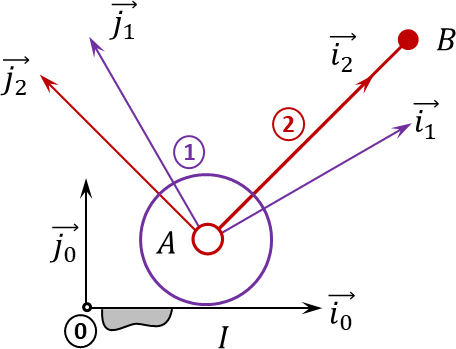
\includegraphics[width=\linewidth]{46_RR_RSG_01}
\end{center}
\fi


\question{Réaliser le paramétrage du mécanisme.}



\ifprof
\else

\footnotesize

\normalsize


\begin{flushright}
\footnotesize{Corrigé  voir \ref{B2:13:PTSI:46}.}
\end{flushright}%
\fi